%
%===============>>  ГРУППА 11-1 МОДУЛЬ 5  <<=============
%
\setmodule{5}

%BEGIN_FOLD % ====>>_____ Занятие 1 _____<<====
\begin{class}[number=1]
	\begin{listofex}
		\item Занятие 1
	\end{listofex}
\end{class}
%END_FOLD

%BEGIN_FOLD % ====>>_____ Занятие 2 _____<<====
\begin{class}[number=2]
	\begin{listofex}
		%1
		\item Материальная точка движется прямолинейно по закону \(x(t) = 6t^2 - 48t + 17\) (где \(x\)  — расстояние от точки отсчета в метрах, \(t\)  — время в секундах, измеренное с начала движения). Найдите ее скорость (в м/с) в момент времени \(t  =  9\) с.
		%2
		\item Материальная точка движется прямолинейно по закону \(x(t) = -t^4 + 6t^3 + 5t + 23\) (где \(x\)  — расстояние от точки отсчета в метрах, \(t\)  — время в секундах, измеренное с начала движения). Найдите ее скорость в (м/с) в момент времени \(t = 3\) с.
		%3
		\item
		\begin{minipage}[t]{\bodywidth}
			На рисунке изображен график функции \( y = f(x)\), определенной на интервале \((-5; 5)\). Найдите количество точек, в которых касательная к графику функции параллельна прямой \(y  =  6\) или совпадает с ней.
		\end{minipage}
		\hspace{0.02\linewidth}
		\begin{minipage}[t]{\picwidth}
			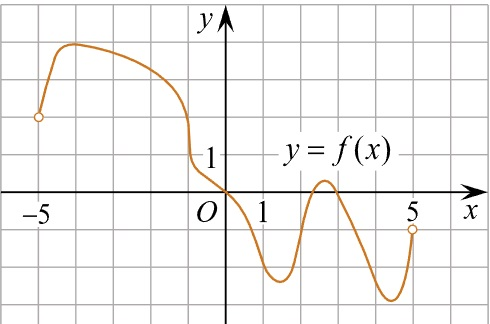
\includegraphics[align=t, width=\linewidth]{\picpath/G111M5L2-1}
		\end{minipage}
		%4
		\item
		\begin{minipage}[t]{\bodywidth}
			На рисунке изображен график производной функции \(f(x)\), определенной на интервале \((-10; 2)\). Найдите количество точек, в которых касательная к графику функции \(f(x)\) параллельна прямой \(y = -2x - 11\) или совпадает с ней.
		\end{minipage}
		\hspace{0.02\linewidth}
		\begin{minipage}[t]{\picwidth}
			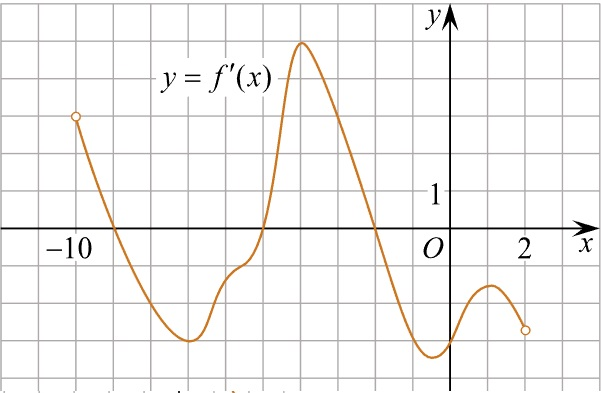
\includegraphics[align=t, width=\linewidth]{\picpath/G111M5L2-2}
		\end{minipage}
		%5
		\item
		\begin{minipage}[t]{\bodywidth}
			На рисунке изображен график производной функции \(f(x)\) , определенной на интервале \( (-6;6) \) . Найдите промежутки возрастания функции \(f(x)\) . В ответе укажите сумму целых точек, входящих в эти промежутки.
		\end{minipage}
		\hspace{0.02\linewidth}
		\begin{minipage}[t]{\picwidth}
			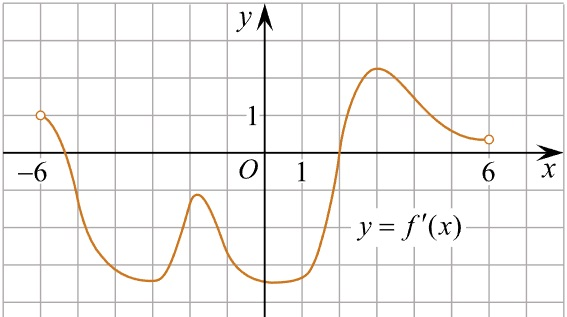
\includegraphics[align=t, width=\linewidth]{\picpath/G111M5L2-3}
		\end{minipage}
		%6
		\item
		\begin{minipage}[t]{\bodywidth}
			На рисунке изображен график функции \(y = f(x)\), определенной на интервале \((-6; 8)\). Определите количество целых точек, в которых производная функции положительна.
		\end{minipage}
		\hspace{0.02\linewidth}
		\begin{minipage}[t]{\picwidth}
			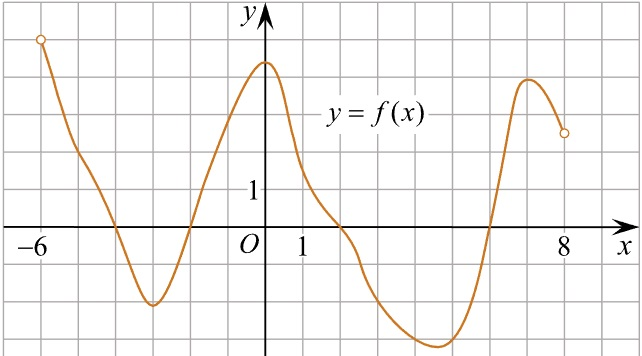
\includegraphics[align=t, width=\linewidth]{\picpath/G111M5L2-4}
		\end{minipage}
		%7
		\item Найдите:
		\begin{itasks}[1]
			\task точку максимума функции \(y = x^3 - 48 + 17\)
			\task наименьшее значение функции \(y = x^3 - 27x\) на отрезке \([0;4]\)
			\task точку максимума функции \(y = x^3 - 5x^2 + 7x -5\)
			\task точку максимума функции \(y = -\dfrac{x^2+289}{x}\)
			\task наименьшее значение функции \(y = \dfrac{x^2+25}{x}\) на отрезке \([1;10]\)
		\end{itasks}
	\end{listofex}
\end{class}
%END_FOLD

%BEGIN_FOLD % ====>>_____ Занятие 3 _____<<====
\begin{class}[number=3]
	\begin{listofex}
		\item В треугольнике \(ABC\) угол \(C\) равен \(90 \degree \), \(AC=4,8\), \(\sin{A} = \dfrac{\sqrt{17}}{17}\). Найдите \(BC\).
		\item В треугольнике \(ABC\) угол \(C\) равен \(90 \degree \), \(AC=2\), \(\cos{A} = 0,5\). Найдите \(AB\).
		\item В треугольнике \(ABC\) угол \(C\) равен \(90 \degree \), \(AC=4\), \(\tan{A} = \dfrac{33}{4\sqrt{33}}\). Найдите \(AB\).
		\item В треугольнике \(ABC\) угол \(C\) равен \(90 \degree \), \(AC=4\), \(BC=7\). Найдите \(\sin{A}\).
		\item В треугольнике \(ABC\) угол \(C\) равен \(90 \degree \), \(CH\) --- высота, \(AB=13\), \(\tg{A} = 5\). Найдите \(BH\).
		\item В треугольник \(ABC, AC = BC = 5\), \( \sin{A}= \dfrac{7}{25} \). Найдите \(AB\).
		\item В треугольник \(ABC, AC = BC, AB = 8\), \( \cos{A}= 0,5 \). Найдите \(AC\).
		\item В треугольник \(ABC, AC = BC = 7\), \( \tg{A}= \dfrac{33}{4 \cdot \sqrt[]{33}} \). Найдите \(AB\).
		\item Найдите:
		\begin{itasks}[1]
			\task точку максимума функции \(y = x^3 - 3x^2 + 2\)
			\task точку максимума функции \(y = (3x^2-36x+36)e^{x+36}\)
			\task наименьшее значение функции \(y = (x+3)^2(x+5)-1\) на отрезке \([-4;-1]\)
			\task наименьшее значение функции \(y = \ln(11x)-11x+9\) на отрезке \(\left[ \dfrac{1}{22};\dfrac{5}{22} \right]\)
		\end{itasks}
	\end{listofex}
\end{class}
%END_FOLD

%BEGIN_FOLD % ====>>_____ Занятие 4 _____<<====
\begin{class}[number=4]
	\begin{listofex}
		\item Один острый угол прямоугольного треугольника на \( 32\degree \) больше другого. Найдите больший острый угол. Ответ дайте в градусах.
		\item Один острый угол прямоугольного треугольника в \( 4 \) раза больше другого. Найдите больший острый угол. Ответ дайте в градусах.
		\item В треугольнике \(ABC\) угол \(C\) равен \(90 \degree \), \(AC=4,8\), \(\sin{A} = \dfrac{7}{25}\). Найдите \(AB\).
		\item В треугольнике \(ABC\) угол \(C\) равен \(90 \degree \), \(AC=2\), \(\cos{A} = \dfrac{\sqrt{17}}{17}\). Найдите \(AC\).
		\item В треугольнике \(ABC\) угол \(C\) равен \(90 \degree \), \(AC=8\), \(\tg{A} = 0,5\). Найдите \(AB\).
		\item В треугольнике \(ABC\) угол \(C\) равен \(90 \degree \), \(CH\) --- высота, \(AB=13\), \(\tan{A} = \dfrac{1}{5}\). Найдите \(AH\).
		\item В треугольнике \(ABC\) угол \(C\) равен \(90 \degree \), \(CH\) --- высота, \(BC=3\), \(\sin{A} = \dfrac{1}{6}\). Найдите \(AH\).
		\item В треугольник \(ABC, AC = BC, AB = 9,6\), \( \sin{A}= \dfrac{7}{25} \). Найдите \(AC\).
		\item В треугольник \(ABC, AC = BC = 8\), \( \cos{A}= 0,5 \). Найдите \(AB\).
		\item В треугольник \(ABC, AC = BC, AB = 8\), \( \tg{A}= \dfrac{33}{4 \cdot \sqrt[]{33}} \). Найдите \(AC\).
	\end{listofex}
\end{class}
%END_FOLD

%BEGIN_FOLD % ====>>_____ Занятие 5 _____<<====
\begin{class}[number=5]
	\begin{listofex}
		\item Занятие 5
	\end{listofex}
\end{class}
%END_FOLD

%BEGIN_FOLD % ====>>_____ Занятие 6 _____<<====
\begin{class}[number=6]
	\begin{listofex}
		\item Занятие 6
	\end{listofex}
\end{class}
%END_FOLD

%BEGIN_FOLD % ====>>_____ Занятие 7 _____<<====
\begin{class}[number=7]
	\begin{listofex}
		\item Основания равнобедренной трапеции равны \(51\) и \(65\). Боковые стороны равны \(25\). Найдите синус острого угла трапеции.
		\item Основания равнобедренной трапеции равны \(43\) и \(73\). Косинус острого угла трапеции равен \(\dfrac{5}{7}\).  Найдите боковую сторону.
		\item Меньшее основание равнобедренной трапеции равно \(23\). Высота трапеции равна \(39\). Тангенс острого угла равен \(\dfrac{13}{8}\).  Найдите большее основание.
		\item Большее основание равнобедренной трапеции равно \(34\). Боковая сторона равна \(14\). Синус острого угла равен \( \dfrac{2\sqrt{10}}{7} \).  Найдите меньшее основание.
		\item Основания равнобедренной трапеции равны \(14\) и \(26\), а ее периметр равен \(60\). Найдите площадь трапеции.
		\item Основания трапеции равны \(18\) и \(6\), боковая сторона, равная \(7\), образует с одним из оснований трапеции угол \(150 \degree \). Найдите площадь трапеции.
		\item Основания трапеции равны \(27\) и \(9\), боковая сторона равна \(8\). Площадь трапеции равна \(72\). Найдите острый угол трапеции, прилежащий к данной боковой стороне
		\item Чему равен больший угол равнобедренной трапеции, если известно, что разность противолежащих углов равна \(50 \degree \)? 
		\item Средняя линия трапеции равна \(28\), а меньшее основание равно \(18\). Найдите большее основание трапеции.
		
		\item Найдите площадь квадрата, если его диагональ равна \(1\).
		\item В параллелограмме \(ABCD, AD  =  3, AD  =  21,  \sin A= \dfrac{6}{7}\).  Найдите большую высоту параллелограмма.
		\item Стороны параллелограмма равны \(9\) и \(15\). Высота, опущенная на первую сторону, равна \(10\). Найдите высоту, опущенную на вторую сторону параллелограмма.
		\item Площадь параллелограмма равна \(40\), две его стороны равны \(5\) и \(10\). Найдите большую высоту этого параллелограмма.
		\item Найдите площадь ромба, если его высота равна \(2\), а острый угол \(30 \degree \).
		\item Сумма двух углов параллелограмма равна \(100\degree \). Найдите один из оставшихся углов.
		
		\item Периметр треугольника равен \(12\), а радиус вписанной окружности равен \(1\). Найдите площадь этого треугольника.
		\item Найдите радиус окружности, вписанной в правильный треугольник, высота которого равна \(6\).
		\item Сторона правильного треугольника равна  корень из 3. Найдите радиус окружности, вписанной в этот треугольник.
		\item Радиус окружности, вписанной в правильный треугольник, равен \(\dfrac{\sqrt{3}}{6}\).  Найдите сторону этого треугольника.
	\end{listofex}
\end{class}
%END_FOLD

%BEGIN_FOLD % ====>>_ Домашняя работа 1 _<<====
\begin{homework}[number=1]
	\begin{listofex}
		%1
		\item Материальная точка движется прямолинейно по закону 
		\[ x(t) = t^2 - 13t + 23, \]
		где \(x\) --- расстояние от точки отсчета в метрах, \(t\) --- время в секундах, измеренное с начала движения. В какой момент времени (в секундах) ее скорость была равна \(2\) м/с?
		%2
		\item
		\begin{minipage}[t]{\bodywidth}
			На рисунке изображён график \(y=f'(x)\)   — производной функции \(f(x)\)  , определенной на интервале \((-8; 3)\). В какой точке отрезка \([-3; 2]\) функция \(f(x)\) принимает наибольшее значение?
		\end{minipage}
		\hspace{0.02\linewidth}
		\begin{minipage}[t]{\picwidth}
			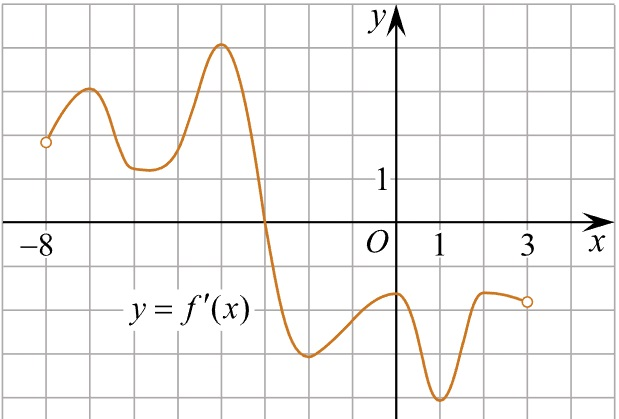
\includegraphics[align=t, width=\linewidth]{\picpath/G111M5H1-1}
		\end{minipage}
		%3
%		\item
%		\begin{minipage}[t]{\bodywidth}
%			На рисунке изображен график производной функции \(f(x)\), определенной на интервале \((-8; 4)\). В какой точке отрезка \([-7; -3] f(x)\) принимает наименьшее значение?
%		\end{minipage}
%		\hspace{0.02\linewidth}
%		\begin{minipage}[t]{\picwidth}
%			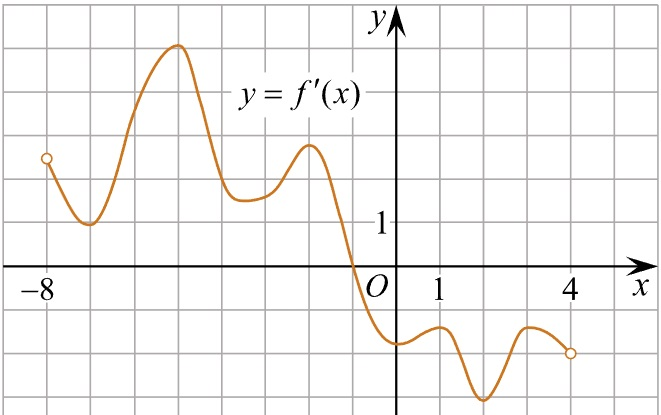
\includegraphics[align=t, width=\linewidth]{\picpath/G111M5H1-2}
%		\end{minipage}
		%4
		\item
		\begin{minipage}[t]{\bodywidth}
			На рисунке изображён график функции \(y=f(x)\) и касательная к нему в точке с абсциссой \(x_0\). Найдите значение производной функции \(f(x)\) в точке \(x_0\).
		\end{minipage}
		\hspace{0.02\linewidth}
		\begin{minipage}[t]{\picwidth}
			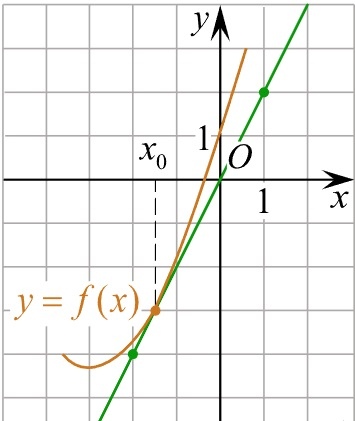
\includegraphics[align=t, width=\linewidth]{\picpath/G111M5H1-3}
		\end{minipage}
		%5
		\item
		\begin{minipage}[t]{\bodywidth}
			На рисунке изображены график функции \(y = f(x)\) и касательная к нему в точке с абсциссой \(x_0\). Найдите значение производной функции \(f(x)\) в точке \(x_0\).
		\end{minipage}
		\hspace{0.02\linewidth}
		\begin{minipage}[t]{\picwidth}
			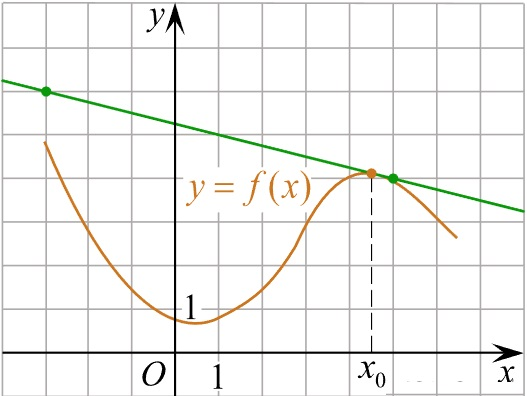
\includegraphics[align=t, width=\linewidth]{\picpath/G111M5H1-4}
		\end{minipage}
		%6
		\item Найдите:
		\begin{itasks}[1]
			\task точку максимума функции \(y = x^3 - 3x^2 + 2\)
			\task наименьшее значение функции \(y = x^3 - 6x^2\) на отрезке \([0;4]\)
			\task точку максимума функции \(y = x^3 + 2x^2 + x + 5\)
			\task точку максимума функции \(y = -\dfrac{x^2+1}{x}\)
			\task наименьшее значение функции \(y = x + \dfrac{36}{x}\) на отрезке \([1;9]\)
%			\task точку максимума функции \( y=-\dfrac{x}{x^2+289} \)
		\end{itasks}
	\end{listofex}
\end{homework}
%END_FOLD

%BEGIN_FOLD % ====>>_ Домашняя работа 2 _<<====
\begin{homework}[number=2]
	\begin{listofex}
		\item В треугольнике \(ABC\) угол \(C\) равен \(90 \degree \), \(CH\) --- высота, \(BC = 8\), \(\sin{A} = 0,5\). Найдите \(BH\).
		\item В треугольнике \(ABC\) угол \(C\) равен \(90 \degree \), \(CH\) --- высота, \(BC=3\), \(\cos{A} = \dfrac{\sqrt[]{35}}{6}\). Найдите \(AH\).
		\item В треугольнике \(ABC\) угол \(C\) равен \(90 \degree \), \(CH\) --- высота, \(BC=5\), \(\cos{A} = \dfrac{7}{25}\). Найдите \(BH\).
		\item В треугольник \(ABC, AC = BC, AB = 8\), \( \sin{BAC}= 0,5 \). Найдите высоту \(AH\).
		\item В треугольник \(ABC, AC = BC, AB = 8\), \( \cos{BAC}= \dfrac{7}{25} \). Найдите высоту \(AH\).
		\item В треугольник \(ABC, AC = BC\), \(AH\) --- высота \( \cos{BAC}= 0,5 \). Найдите высоту \(BH\).
	\end{listofex}
\end{homework}
%END_FOLD

%BEGIN_FOLD % ====>>_ Домашняя работа 3 _<<====
\begin{homework}[number=3]
	\begin{listofex}
		\item Хорда \( AB \) делит окружность на две части, градусные величины которых относятся как \( 1:2 \). Под каким углом видна эта хорда из точки \( C \), принадлежащей меньшей дуге окружности? Ответ дайте в градусах.
		\item Касательные \( CA \) и \( CB \) к окружности образуют угол \( ACB \), равный \( 122\degree \). Найдите величину меньшей дуги \( AB \), стягиваемой точками касания. Ответ дайте в градусах.
		\item Радиус окружности, описанной около правильного треугольника, равен \( \sqrt{3} \). Найдите сторону этого треугольника.
		\item Радиус окружности, описанной около прямоугольного треугольника, равен \( 4 \). Найдите гипотенузу этого треугольника.
		\item Одна сторона треугольника равна радиусу описанной окружности. Найдите острый угол треугольника, противолежащий этой стороне. Ответ дайте в градусах
		\item Два угла вписанного в окружность четырехугольника равны \( 82\degree\) и \( 58\degree \). Найдите больший из оставшихся углов. Ответ дайте в градусах.
	\end{listofex}
\end{homework}
%END_FOLD

%BEGIN_FOLD % ====>>_ Занятие 8 _<<====
\begin{class}[number=8]
	\begin{listofex}
		\item Найдите площадь треугольника, две стороны которого равны \(8\) и \(12\), а угол между ними равен \(30 \degree \).
		\item В треугольнике \(ABC, AD\)  --- биссектриса, угол \(C\) равен \(30 \degree\), угол \(BAD\) равен \(22 \degree\). Найдите угол \(ADB\). Ответ дайте в градусах.
		\item В треугольнике \(ABC\) угол \(C\) равен \(90 \degree \), \(CH\)  --- высота, \(AH = 12\),  \(\cos A = \dfrac{2}{3} \).  Найдите \(AB\).
		\item В треугольнике \(ABC\) угол \(C\) равен \(90 \degree \), высота \(CH\) равна \(20, BC  =  25\). Найдите  синус \(A\).
		\item Основания равнобедренной трапеции равны \(7\) и \(13\), а ее площадь равна \(40\). Найдите периметр трапеции и её боковую сторону.
		\item Найдите площадь прямоугольной трапеции, основания которой равны \(6\) и \(2\), большая боковая сторона составляет с основанием угол \(45 \degree\).
		\item Основания трапеции равны \(18\) и \(6\), боковая сторона, равная \(7\), образует с одним из оснований трапеции угол \(150 \degree \). Найдите площадь трапеции.
		\item Найдите площадь прямоугольной трапеции, основания которой равны \(6\) и \(2\), большая боковая сторона составляет с основанием угол \(45 \degree \).
		
		\item Периметр прямоугольника равен \(34\), а площадь равна \(60\). Найдите диагональ этого прямоугольника.
		\item Найдите периметр прямоугольника, если его площадь равна \(18\), а отношение соседних сторон равно \(1:2\).
		\item Периметр прямоугольника равен \(28\), а диагональ равна \(10\). Найдите площадь этого прямоугольника.
		\item Один угол параллелограмма больше другого на \(70 \degree \). Найдите больший угол.
		\item Диагональ параллелограмма образует с двумя его сторонами углы \(26\degree\) и \(34\degree \). Найдите больший угол параллелограмма.
		\item Периметр параллелограмма равен \(46\). Одна сторона параллелограмма на \(3\) больше другой. Найдите меньшую сторону параллелограмма.
		
		\item Радиус окружности, вписанной в правильный треугольник, равен \(6\). Найдите высоту этого треугольника.
		\item Сторона ромба равна \(1\), острый угол равен \(30\) градусов. Найдите радиус вписанной окружности этого ромба.
		\item Острый угол ромба равен \(30\degree \). Радиус вписанной в этот ромб окружности равен \(2\). Найдите сторону ромба.
		\item Найдите сторону правильного шестиугольника, описанного около окружности, радиус которой равен \(\sqrt{3}\).
		
		\item Точки \(A, B, C,\) расположенные на окружности, делят ее на три дуги, градусные величины которых относятся как \(1 : 3 : 5\). Найдите больший угол треугольника \(ABC\). Ответ дайте в градусах.
		\item Угол \(A\) четырехугольника \(ABCD\), вписанного в окружность, равен\(58 \degree \). Найдите угол \(C\) этого четырехугольника.
		\item Стороны четырехугольника \(ABCD\) --- \(AB, BC, CD и AD\) стягивают дуги описанной окружности, градусные величины которых равны соответственно \(95\degree \), \(49\degree\), \(71\degree\), \(145\degree\). Найдите все углы этого четырехугольника.
	\end{listofex}
\end{class}
%END_FOLD
